% !TeX root = ../main.tex
\chapter{测量平台设计与搭建}



\section{总体设计}\label{sec:rig-overall}

根据上文规划的测量方案以及实际需求,设计大气环境下的静电卡盘静电力检测平台,希望能达成如下目标:

\begin{enumerate}
  \item 实现用背吹平衡 -- 微力探头法检测静电力
  \item 自动化检测过程,减小人为误差
  \item 采集检测过程中各关键变量,方便后续数据处理与分析
\end{enumerate}

下面将详细阐述测量平台的设计方案。


\subsection{测量平台组成}\label{sec:rig-overall-comp}

\begin{figure}[tbh]
\centering
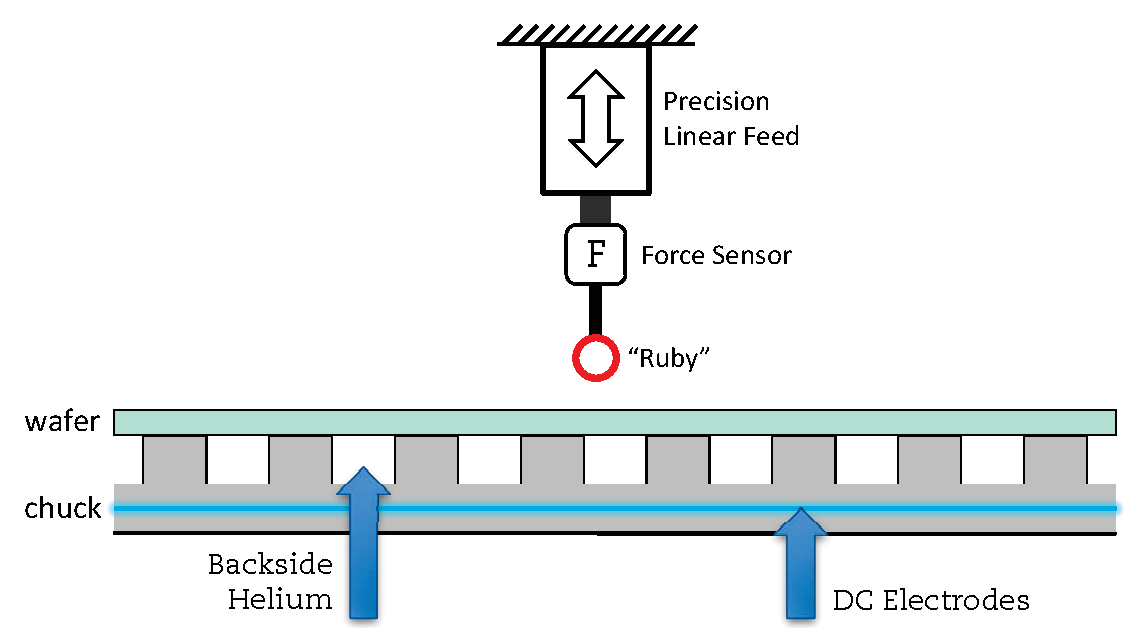
\includegraphics[width=1\linewidth]{rig/overall__sch}
\caption{测量平台总体设计示意}
\label{fig:rig-overall-sch}
\end{figure}

如图~\ref{fig:rig-overall-sch},整个测量平台由以下组件构成:

\begin{itemize}
  \item 待测静电卡盘及其配套静电电源
  \item 微力探头组件
  \item 背吹控制系统
  \item 机械结构
  \item 电控与数据采集系统
\end{itemize}

除静电卡盘与电源外,其他组件均需自行设计、搭建。


\subsection{检测流程}\label{sec:rig-overall-proc}

一次完整的检测过程分如下步骤完成:

\begin{enumerate}
  \item 准备静电卡盘
  \begin{enumerate}
    \item 用无水乙醇擦拭静电卡盘与晶圆
    \item 将晶圆小心地放置在静电卡盘陶瓷层正中央
    \item 开启静电电源,调节电极电压至目标电压
  \end{enumerate}
  
  \item 准备测量平台
  \begin{enumerate}
    \item 降下微力探头,使其轻轻接触晶圆
    \item 确认背吹控制系统中调压装置均处于零位
  \end{enumerate}
  
  \item 检测
  \begin{enumerate}
    \item 开始自动记录微力探头受力、背吹入口气压两变量
    \item 背吹气压接通并缓慢、均匀地上升
    \item 当微力探头受力即将达到其满量程时,自动切断背吹气压,检测停止
  \end{enumerate}
  
  \item 后续处理
  \begin{enumerate}
    \item 导出采集到的数据
    \item 微力探头复位上升
    \item 切断静电电源,短接两电极引线,消除部分残余电荷
    \item 小心将晶圆取下
  \end{enumerate}
\end{enumerate}



\clearpage



\section{微力探头组件设计}\label{sec:rig-probe}

图~\ref{fig:rig-overall-sch}中,卡盘上方的组件即为微力探头组件微力探头组件,其在\ref{principle-gap-ruby}节中提到的微力传感器和红宝石探头的基础上,增设精密直线进给机构:固定端连接在框架上,移动端与力传感器的固定端相连,用于驱动探头沿z方向移动,以实现“轻轻接触晶圆”这一动作。


\subsection{微力传感器选型}\label{sec:rig-probe-sensor}

微力传感器是探头组件中的核心元件,因此优先选型。考虑到其在测量系统中的作用,主要关心以下参数:

\begin{enumerate}
  \item \textbf{量程}:
    无论在轻触阶段还是在脱附检测阶段,探头均不应向晶圆施加过大的力。粗估静电力处于$\SI{10}{\newton}$至$\SI{200}{\newton}$之间,探头施加的力应低于其$1 ~\%$,即微力传感器应能准确测量 大致在$\SI{0.1}{\newton}$至$\SI{2}{\newton}$范围内的单轴压缩力。
  \item \textbf{分辨力}:
    微力传感器需能检测到微小的受力变化,根据上述关于量程的讨论,应能至少分辨出$\SI{1}{\milli\newton}$的力增量。不同的传感器可能对分辨力的标称方法不同,应结合其输出信号特点,判定其是否满足要求。
  \item \textbf{刚度}:
    微力传感器的敏感端存在一位移,一般服从胡克定律,与受力成比例关系。\ref{principle-gap}节中讨论了晶圆与卡盘间气隙可能对静电力产生的影响。若传感器刚度较高,则可更好地控制气隙大小,并在气隙明显扩大之前检测出脱附;但另一方面,高刚度使轻触晶圆更难实现(见\ref{sec:rig-probe-feeding}节\eqref{eq:rig-probe-feeding-vel}式)。因此该参数并无明确要求,仅做为选型时的参考。
  \item \textbf{过载能力}:
    考虑到在安装、调试过程中,以及硅晶圆突然完全脱附时,探头均可能瞬间受到较大的力的作用;若微力传感器承受过载能力较好,则可避免其意外受损。
\end{enumerate}

初步筛选市面上各种微力传感器得到表~\ref{tab:rig-probe-sensor}。若考虑量程、精度、分辨力,1050V1较差;若考虑刚度,LSB200较差;若考虑过载性能,FT-S10000较差。由上文讨论,量程、分辨力是最重要的性能指标,而刚度因素较为次要,且即使是刚度最低的LSB200,其值也已达到$\SI[per-mode=symbol]{1}{\milli\newton\per\micro\meter}$,因此选择LSB200型应变式微力传感器。

% generated using http://www.tablesgenerator.com/latex_tables
\begin{table}[htbp]
\begin{minipage}{1\linewidth}
\centering
\caption{微力传感器选型表}
\label{tab:rig-probe-sensor}
\begin{tabular}{@{}lllccc@{}}
\toprule[1.5pt]
生产商 &  &  & Futek & Dytran & FemtoTech \\
型号 &  &  & LSB200 & 1050V1 & FT-S10000 \\
\midrule[1pt]
原理 &  &  & 应变式 & 压电式 & MEMS \\
输出信号 & 类型 &  & 电阻电桥 & 电压 & 电压 \\
 & 单位 &  & $\si[per-mode=symbol]{\milli\volt\per\volt}$ & V & V \\
灵敏度 & 满量程 & 输出 & 0.5 & 5 & 2 \\
 & 单位受力 & 输出/$\si{\newton}$ & 5.0E+00 & 1.1E-01 & 2.0E+02 \\
分辨力 &  & $\si{\micro\newton}$ & --\footnote{未标称,下同} & 600 & 0.5 \\
刚度 &  & $\si[per-mode=symbol]{\newton\per\micro\meter}$ & 0.001 & 1996.45 & -- \\
\midrule[1pt]
满量程 & 拉(+) & $\si{\newton}$ & 0.1 & 44.48 & 0.01 \\
 & 压(-) & $\si{\newton}$ & 0.1 & 44.48 & 0.01 \\
最大载荷 & 拉(+) & $\si{\newton}$ & 1 & 889.64 & 0.03 \\
 & 压(-) & $\si{\newton}$ & 1 & 889.64 & 0.03 \\
\midrule[1pt]
线性度 &  & \% FS & 0.1 & 1 & \multirow{2}{*}{--} \\
 &  & $\si{\newton}$ & 2.00E-04 & 8.90E-01 &  \\
滞回 &  & \% FS & 0.1 & \multirow{2}{*}{--} & \multirow{2}{*}{--} \\
 &  & $\si{\newton}$ & 2.00E-04 &  &  \\
重复精度 &  & \% FS & 0.05 & \multirow{2}{*}{--} & \multirow{2}{*}{--} \\
 &  & $\si{\newton}$ & 1.00E-04 &  &  \\
\bottomrule[1.5pt]
\end{tabular}
\end{minipage}
\end{table}


\subsection{进给机构选型}\label{sec:rig-probe-feeding}

进给机构的主要作用为完成“轻触晶圆”动作,其移动组件可为推杆或直线滑移台(优先推杆),驱动方式可为手动或电动(优先电动)。对于手动进给机构,只需考虑其最小步长(受静摩擦等因素限制),因此下面主要讨论电动进给机构的选型。主要关心以下参数:

\begin{enumerate}
  \item \textbf{低速性能}:
    由于当探头接触到晶圆时,接触力会突增,为了限制接触力,需要控制探头以较低速度接近晶圆,直至微力传感器读数出现明显变化,即命令进给机构停止运动。这要求进给机构能够在低速下平稳运行,即低速速度波动较小,或爬行现象不明显。参考运动速度可按\eqref{eq:rig-probe-feeding-vel}计算:
    \begin{equation}
    \label{eq:rig-probe-feeding-vel}
    v_{\mathrm{ref}} = \frac{ F_{\mathrm{thres}} }
                            { k_{\mathrm{sensor}} \cdot t_{\mathrm{delay}} }
    \end{equation}
    其中:
    \begin{itemize}
      \item $F_{\mathrm{thres}}$  : 探头接触晶圆时最大允许施加的力
      \item $k_{\mathrm{sensor}}$ : 微力传感器刚度
      \item $t_{\mathrm{delay}}$  :  从探头受力跳变到进给机构停止运动的总时滞(包括机械惯性、信号传输延迟等)
    \end{itemize}
    代入LSB200相关数据(
    $F_{\mathrm{thres}} = \SI{1}{\milli\newton}$,
    $k_{\mathrm{sensor}} = \SI[per-mode=symbol]{0.001}{\newton\per\micro\meter}$
    ),在$t_{\mathrm{delay}} = \SI{0.01}{\second}$时计算参考速度为$\SI[per-mode=symbol]{100}{\micro\meter\per\second}$。
  \item \textbf{总行程}:
    小型精密电动进给机构行程较低,可采用粗精二级调节的方法:先用手动或电动方式粗调整个微力探头组件,将其固定在接近晶圆的位置上,再驱动精密进给机构完成轻触动作。为了方便粗调,希望总行程至少为$\SI{5}{\milli\meter}$。
  \item \textbf{背隙/回差/抖动}:
    完成轻触晶圆动作后,进给机构需保持原位不动(锁定),因此对于能够自锁的机构,不应有回差影响;对于不能自锁的机构,需确认其因反馈控制产生的抖动在合理范围内。
\end{enumerate}

由于候选型号较多,完整的选型表参见附录B。 %TODO:xref appendix
最终选定的电动进给机构为LAC10A-T4精密电动推杆,其原理为步进电机驱动滚珠丝杠,有效行程$\SI{10}{\milli\meter}$,重复定位精度$\pm\SI{1.5}{\micro\meter}$,具有自锁特性。



\clearpage



\section{背吹控制系统设计}\label{sec:rig-pressure}

背吹平衡法需要控制静电卡盘背吹入口压强\footnotemark{}缓慢、平稳上升,并实时测量、记录该压强数值;最好还能同时测出进入背吹通道的流量。显然,整个系统可分为供压与传感两部分,关键参数为压强、流量。
%TODO:cite力大小来源,最好北方微电子
按照待测静电卡盘的参数($d = \SI{296}{\milli\meter}$,$F \leq \SI{200}{\newton}$,压强等效面积定为 总面积$1/2$)估算,背吹入口压强最大不会超过$\SI{6}{\kilo\pascal}$。由于之前尚未有在大气环境下针对类似尺寸的静电卡盘的背吹试验,流量范围未知,需通过实测获得。

\footnotetext{由于测量平台处于大气环境下,所有压强均为表压(相对于大气压强),下略。}


\subsection{供压方案分析}\label{sec:rig-pressure-supply}

常见的气压控制元件主要应用于气动机械(如气缸、气爪、气动回转台等),压强下限一般为$\SI{0.1}{\mega\pascal}$级,与系统要求差距很大,因此需仔细拟定气压控制方案,选择合适的组件保证气压精确控制。

\subsubsection{集成电子压强控制单元}\label{sec:rig-pressure-supply-integrated}

这类产品集成了压强控制所需的所有电、气元件,接受一个电信号输入作为压强设定点,控制出口压强等于该设定点。其中,部分产品包括完整的显示、操作单元、通信接口等,如WIKA CPC2000/CPC6000压强控制器等(图~);部分产品只有简单的指示器,设定点为模拟信号(如$\num{4} \sim \SI{20}{\milli\ampere}$信号),如TESCOM ER3000/ER5000系列、SMC ITV00x0系列电子比例阀等。完整的压强控制器较为昂贵,但精度较高,量程可选余地较大;电子比例阀成本较低,但其量程一般仍为气动机械级,而其小量程型号允许的流量过低(如SMC ITV0010型,最低输出压强$\SI{1}{\kilo\pascal}$,最大流量仅$\SI[per-mode=symbol]{3.5}{\liter\per\minute}$)。

\begin{figure}[tbh]
\centering
\includegraphics[width=0.75\linewidth]{rig/pressure__supply__cpc6000.png}
\caption{WIKA CPC6000压强控制器}
\label{fig:rig-pressure-supply-cpc6000}
\end{figure}

\subsubsection{反馈控制微型气泵}\label{sec:rig-pressure-supply-pump}

参考CPC2000的工作原理示意图(图~\ref{fig:rig-pressure-supply-cpc2000-sch}),可用独立元件设计类似的压强控制系统,如图~\ref{fig:rig-pressure-supply-pump-sch}:使用直流电机驱动的微型气泵作为压力源,压强变送器提供反馈信号,闭环PI控制气泵输出功率。为减小气泵固有的压强波动,可采取如下措施:

\begin{enumerate}
  \item 在泵与背吹通道入口间增设双端气瓶,通过增加惯性环节的方式降低压强波动;
  \item 在背吹通道入口处加设一节流阀通向大气,避免电机反复启停造成的压强波动;
\end{enumerate}

\begin{figure}[tbh]
\centering
\includegraphics[width=1\linewidth]{rig/pressure__supply__cpc2000__sch.png}
\caption{CPC2000工作原理示意}
\label{fig:rig-pressure-supply-cpc2000-sch}
\end{figure}

\begin{figure}[tbh]
\centering
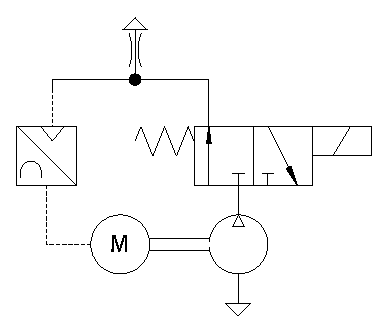
\includegraphics[width=0.618\linewidth]{rig/pressure__supply__pump__sch}
\caption{反馈控制微型气泵示意}
\label{fig:rig-pressure-supply-pump-sch}
\end{figure}

\subsubsection{精密机械式减压阀}\label{sec:rig-pressure-supply-reg}

机械式减压阀的原理是通过膜片平衡,反馈控制小孔开度,从而达到稳定输出压强的目的。即便是原本应用于气动机械的精密减压阀,根据其原理不同,有些产品允许出口压强低于其标称最低输出压强,只不过此时输出压强随流量改变。如SMC IR1000型精密减压阀(图~\ref{fig:rig-pressure-supply-ir1000}),标称调压范围$\num{5} \sim \SI{200}{\kilo\pascal}$,标称灵敏度$\SI{0.4}{\kilo\pascal}$。除了可用作电子比例阀的前置减压阀外,有可能直接接入背吹通道,作为小开度节流阀使用,提供$\num{0} \sim \SI{5}{\kilo\pascal}$范围内的缓慢变化的压强。
%TODO:xref rig test and indicate

\begin{figure}[tbh]
\centering
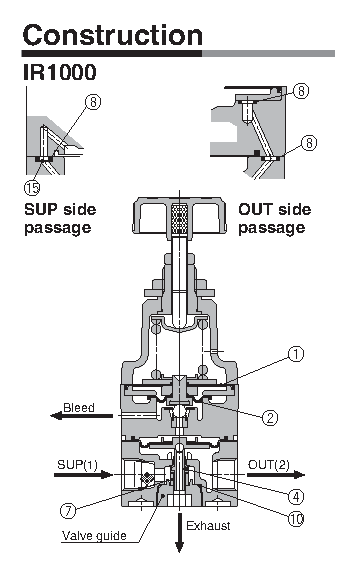
\includegraphics[height=0.9\textheight]{rig/pressure__supply__IR1000}
\caption{IR1000简化剖视}
\label{fig:rig-pressure-supply-ir1000}
\end{figure}


\subsection{传感部分选型}

无论供压部分采用何种方案,均不影响压强传感器的选型。完整的选型表见附录B。 %TODO:xref appendix
最终选定Honeywell STD720精密差压变送器(量程可在$\pm \num{1} \sim \pm \SI{100}{\kilo\pascal}$范围内任意配置,基础准确度$0.05\%$,输出$\num{4} \sim \SI{20}{\milli\ampere}$模拟信号、HART现场总线协议)。另外配置$\SI{16}{\kilo\pascal}$量程的机械指针式压强计,辅助调试。



\clearpage



\section{机械结构设计}\label{sec:rig-model}

根据图~\ref{fig:rig-overall-sch},设计测试平台的机械结构。为了方便加工、搭建,选用标准$\num{30} \times \SI{30}{\milli\meter}$系列开槽铝合金型材及配套标准连接件,与依据待测静电卡盘的外形尺寸设计的连接板共同构成框架结构;其他组件均通过连接件与之相连。框架结构的简化三维模型如图~\ref{fig:rig-model-all-iso}\footnote{型材连接部分零件数较多,因此并未全部在总装配体三维模型中表示出。}。

\begin{figure}[p]
\centering
\includegraphics[width=1\textwidth]{rig/model__all__iso.png}
\caption{测试平台装配体三维模型}
\label{fig:rig-model-all-iso}
\end{figure}


\subsection{静电卡盘连接板}\label{sec:rig-model-base}

该连接板位于整个测试平台中心,其尺寸与配合特征主要由静电卡盘决定,并间接决定了整个框架的尺寸。静电卡盘通过螺钉紧固在连接板上,因此连接板需提供相配合的螺纹孔与承载面。如图~\ref{fig:rig-model-echuck-back}\footnotemark{},静电卡盘的底部有多个功能特征,除氦气背吹接口需特殊设计外,其他特征(如直流电极接口、顶针孔等)均需裸露在外以正常使用,因此连接板上对应位置开槽。氦气背吹接口并未采用常见的螺纹连接方式,而是一$\diameter{}4$光孔,需设计密封接头与之相连。如图~\ref{fig:rig-model-echuck-plug-assy},用三个紧定螺钉使密封接头上表面与卡盘背面紧密配合,通过标准O型圈形成端面密封,其另一端提供M5内螺纹,与标准气动快装接头连接,方便配管。

\footnotetext{北方微电子公司内部图纸,仅保留轮廓与功能描述。}

\begin{figure}[tbhp]
\centering
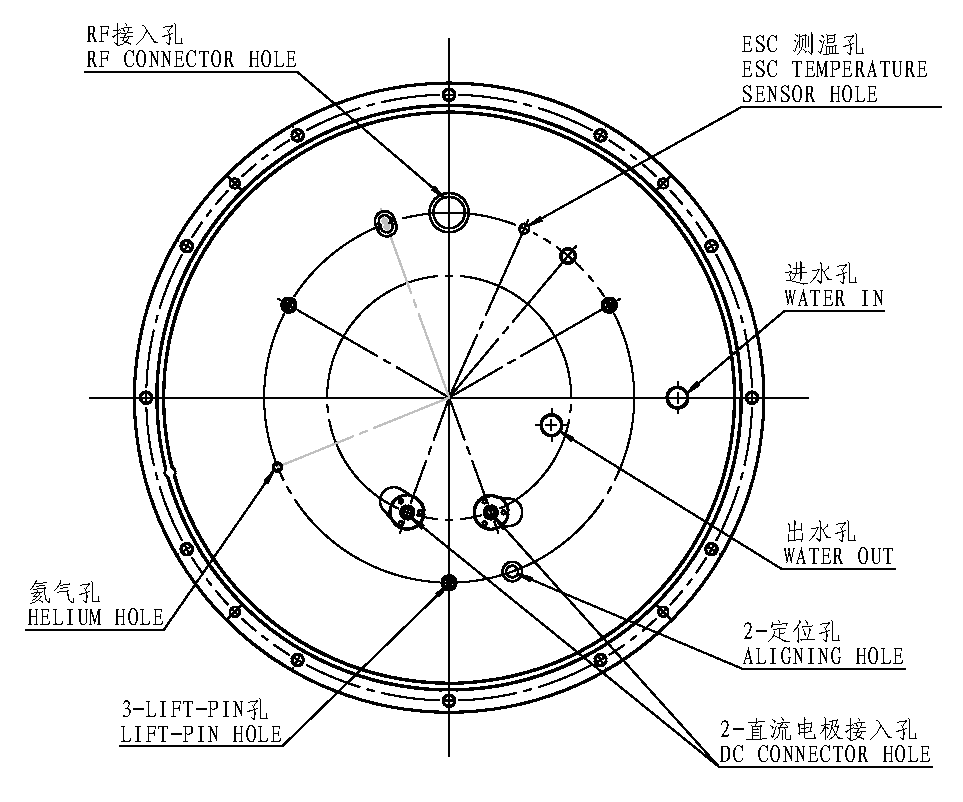
\includegraphics[height=0.45\textheight]{rig/model__echuck__back}
\caption{静电卡盘背面特征工程图}
\label{fig:rig-model-echuck-back}
\end{figure}

\begin{figure}[tbhp]
\centering
\includegraphics[height=0.45\textheight]{rig/model__echuck__plug__assy2}
\caption{端面密封设计工程图}
\label{fig:rig-model-echuck-plug-assy}
\end{figure}


\subsection{型材框架结构}\label{sec:rig-model-frame}

框架主体为三层对称结构:中间一层是静电卡盘连接板,上下各用4根型材连接成正方形(型材间使用铸钢角件和紧定螺钉连接);层与层之间用4根纵向型材负责承重,在连接板侧使用$\num{50}\times\num{50}\times\SI{30}{\milli\meter}$挤压角件连接(三维模型中已表示出),在正方形型材侧使用$\num{60}\times\num{60}\times\SI{30}{\milli\meter}$角件连接。这种连接方式的主要优点是不依靠型材与角件的摩擦力承受重量,而是靠型材、角件、连接螺栓将载荷传至地面。

框架主体以外,还有2根型材组成的简易手动定位结构,用于连接微力探头,其横梁通过T型螺母、普通螺栓、大垫圈紧固在最上层正方形的下侧,竖梁使用$\num{60}\times\num{60}\times\SI{30}{\milli\meter}$角件连接在横梁上。通过改变这2根型材连接位置,即可改变微力探头在晶圆平面上的投影位置。


\subsection{微力探头装配}\label{sec:rig-model-probe}

%TODO:refine description -- in more detail

如图~\ref{fig:rig-model-probe},设计连接板,将微力探头组件\footnotemark{}通过沉头螺钉固定在其上;若选择使用电动推杆,需先使用自带的六角薄螺母固定在图示连接块上。连接板后部设导向键,配合T型螺母、内六角螺栓连接在型材上。

由于此处空间较小,还有较为敏感的微力传感器(最大承受$\SI{1}{\newton}$力),应特别注意装配顺序:

\begin{enumerate}
  \item
    传感器处于平放状态(贴有商标一面向上),轻轻握住传感器活动端,小心将红宝石探头(需加M2$\to$M3转接头)旋入、拧紧;
  \item
    使手动平移台/电动推杆处于伸长状态,轻轻握住传感器固定端,将其连接在平移台/推杆上。
  \item
    手持平移台/推杆,将其通过沉头螺钉固定在连接板上。
\end{enumerate}

\footnotetext{三维模型中两组微力探头是为了同时在图中表示手动和电动两种情况下的连接方式,实际仅选装一组。}

\begin{figure}[tbhp]
\centering
\includegraphics[height=0.45\textheight]{rig/model__probe.png}
\caption{探头组件数字模型}
\label{fig:rig-model-probe}
\end{figure}



\clearpage



\section{电控与数据采集系统设计}\label{sec:rig-ctrl}

为了实现检测过程自动化,减小人操作对结果产生的干扰,设计电控与数据采集系统。检测平台中所有电子模块及其信号流动关系如图~\ref{fig:rig-ctrl-sch}。

\begin{figure}[tbhp]
\centering
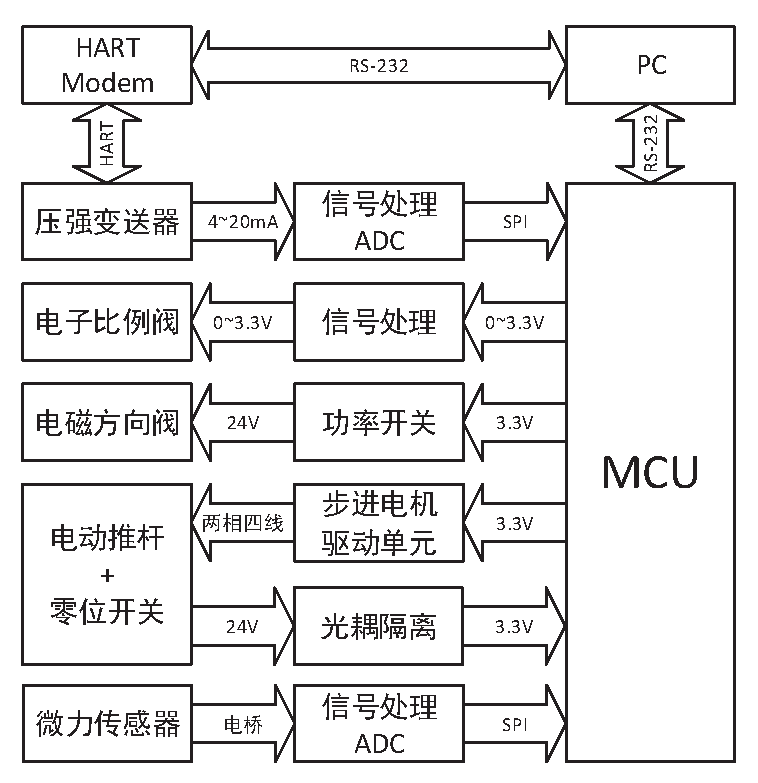
\includegraphics[height=0.5\textheight]{rig/ctrl__sch}
\caption[电控系统框图]{电控与数据采集系统模块框图}
\label{fig:rig-ctrl-sch}
\end{figure}




\section{搭建与调试}\label{sec:rig-build}